\documentclass[twocolumn,12pt]{article}

\textheight 9 in
\voffset -.75 in

\usepackage{amssymb}
\usepackage{amsmath}
\usepackage{bm}
\usepackage{graphicx}
\usepackage{epstopdf}
\usepackage{hyperref}
\usepackage{natbib}
\usepackage{tikz}
\usepackage{fancyhdr}
\usepackage{algpseudocode}
\usepackage{algorithm}
\usepackage[toc,page]{appendix}

\setlength{\parskip}{5pt plus1pt minus1pt}

\DeclareMathSizes{36}{36}{36}{36}

\title{Train Harder, Smarter:\\Using Graph Theory to Create Route Suggestions}
\author{Forest Trimble\\trimbf@rpi.edu}
\begin{document}

\setlength{\headheight}{15pt}

\pagestyle{fancy}
\fancyhead{}
\fancyhead[L]{Forest Trimble}
\fancyhead[R]{Train Harder, Smarter}
\maketitle

\newcommand{\mycite}[1]{[\citenum{#1}]}

\begin{abstract}
  \emph{Cyclists are always in search of the perfect ride on the perfect
  roads. They have criteria like distance and elevation gain to ensure
  that they get in the workout that they want. Unfortunately, to
  find this ideal ride manually, it takes a great deal of exploring and
  time, and eventually, one may settle into the habit of using the same
  roads that he/she already knows. We research a way to improve this
  paradigm, and to generate cyclists exactly the route they are looking
  for, without them having to do any work.}
\end{abstract}

\section{Background} \label{sec:back}

Cycling can be wildly different based on the roads that one takes: On busy
roads with no shoulders, it can be borderline miserable, while few things in
the world are better than spinning down a smoothly paved road with beautiful
vistas of open countryside and no traffic. Unfortunately, cyclists need to
invest massive amounts of time and energy exploring the roads and amassing a
repertoire that they can use. Additionally, it is difficult to satisfy criteria
for training, like an elevation gain and distance, using only that mental
repertoire. This paper chronicles the attempt to unroll a solution for this
problem.

Specifically, a good solution should take as input a distance to travel, a
start point, and, optionally, an elevation gain, and generate a route from the
start point that satisfies the distance and elevation gain within some
tolerance. A fully robust solution would also utilize user data to ensure that
it traverses the most pleasant roads to ride on and avoids the worst.

\section{Tools}

Creating a solution to this problem from scratch is unnecessary. The larger part
of this problem has already been solved: maps have been digitized and
parsers for the data format already exist. This section details the various
tools and technologies that the algorithm leverages.

First and foremost, we opted to use the Open Street Map format, which is open
source, fairly robust, and has a very active community that contributes to both
the maps themselves and to various (mostly open-source) software projects that
utilize the format. The interested reader should refer to \citenum{wik:osm} for
almost all information regarding OSM, including how to contribute, how to use,
and links to projects that utilize OSM instead of proprietary mapping software.

Additionally, we leveraged some existing code to more easily be able to create
a demonstrable algorithm. Pyroute was used, since it has the very nice feature
that the navigation component was entirely decoupled into PyrouteLib. This
allows easy utilization of the Pyroute tools for GUI setup and OSM download
while also making it rather explicit where the navigation functions are.
Notably, pyroute has generally been abandoned in favor of the more advanced
Open Source Routing Machine (OSRM) project, but pyroute was chosen for this
paper instead due to its relative ease of prototyping and intuitiveness. Readers
interested in OSRM should refer to \mycite{wik:osrm}; those interested in
pyroute can sate their interest with \mycite{wik:pyroute}. One notes that
pyroute uses the relatively simple $A^*$ algorithm for routing between two
points. This is a slower implementation than OSRM, but our usage of the actual
routing algorithm is minimal; for the most part, we use pyroute only for loading
maps and displaying routes on them.

\section{Algorithm}

The core idea of our algorithm
is that at any point along the route, the engine generates weights for each
different possible direction to take, generates a random number, and picks a
direction according to the random number and the weights. There are several
different ideas that are competing for weight, so we'll break it down into the
individual components first, and then describe the combination at the end.

Additionally, the algorithm requires a few inputs from the user (in addition
to the Open Street Map network of roads):
\begin{itemize}
\item A distance to travel, $d$.
\item A direction in which to head $\phi$.
\item An elevation to gain, $h$.
\item A start point, $x_0$.
\end{itemize}

\subsection{Weight for Distance}

\begin{figure}
  \centering
  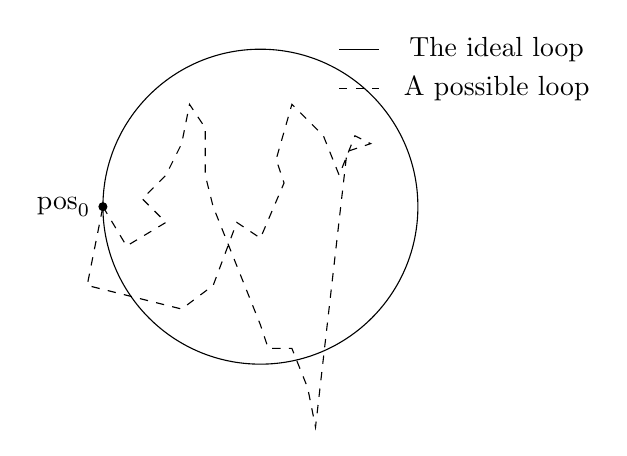
\begin{tikzpicture}
    \node (init) at (-0.5,0) {$\mbox{pos}_0$};
    \filldraw (0,0) circle(0.05);

    \draw (2,0) circle(2);
    \draw[dashed] (0,0) -- (0.3,-.5) -- (0.8,-0.2) -- (0.5,0.1) -- (0.8,0.4) --
    (1.0,0.8) -- (1.1,1.3) -- (1.3,1.0) -- (1.3,0.4) -- (1.4, 0) -- (1.6, -0.5)
    -- (1.8, -1) -- (2.0,-1.5) -- (2.1,-1.8) -- (2.4,-1.8) -- (2.6,-2.3) --
    (2.7,-2.8) -- (3.1,0.7) -- (3.4,0.8) -- (3.2,0.9) -- (3.0,0.4) -- (2.8,0.9)
    -- (2.4,1.3) -- (2.2,0.6) -- (2.3,0.3) -- (2.0,-0.4) -- (1.7, -0.2) --
    (1.4,-1) -- (1.0,-1.3) -- (-0.2,-1) -- (0,0);

    \node (mainleg) at (5,2) {The ideal loop};
    \node (altleg) at (5,1.5) {A possible loop};
    \draw (3,2) -- (3.5,2);
    \draw[dashed] (3,1.5) -- (3.5,1.5);
  \end{tikzpicture}
  \caption{The ideal loop starting at $\mbox{pos}_0$ contrasted with a possible
    actual loop} \label{fig:ideal}
\end{figure}

The first weight is based on distance. The idea is that there is a theoretical,
perfect loop that covers exactly the amount of distance that you would like,
and the algorithm does its best to direct you along that loop. See
Figure~\ref{fig:ideal} for an example of what this might look like. In order to
direct you along this loop, weights are generated based on
direction. We'll consider the method for finding the optimal direction,
$\theta$.


\subsubsection{Calculating the Weights}

\begin{figure}
  \centering
  \begin{tikzpicture}
    \node (theta) at (0,4.2) {$\theta$};


    \node (max) at (0.2,3) {2};
    \node (min) at (0.35,1) {0.5};
    \node (avg1) at (-1,2.2) {1};
    \node (avg2) at (1,2.2) {1};

    \draw[thick,<->] (0,0) -- (0,4);
    \draw[thick,<->] (-2,2) -- (2,2);
  \end{tikzpicture}
  \caption{A possible weighted compass} \label{fig:weights}
\end{figure}

First, consider how the weights are generated once
that direction is discovered. Basically, there is a weighted compass oriented
along $\theta$, with weights from 0.5 to 2. See Figure~\ref{fig:weights} to
see what we mean. As shown, the weights do not scale linearly. Instead, they
scale exponentially. This ensures that the weights are mostly centered around
the perpendicular, with growth accelerating farther from the perpendicular.
The idea is to have the weight be double in the ideal
direction, half moving exactly opposite the ideal direction, and unchanged
perpendicular to the ideal direction. Considering these three pieces of
information, we are looking for some $f : [0,2\pi] \to [0.5,2]$ as follows:
\begin{align*}
  2 = & f(\theta) \\
  1 = & f(\theta \pm \frac{\pi}{2}) \\
  \frac{1}{2} = & f(\theta \pm \pi)
\end{align*}
Let $\tau$ be the angle under consideration. We let
\[ \mbox{ang}(\tau, \theta) = |\theta - \tau \mbox{ mod } \pi|. \]
This allows us to define $f$ in terms of the angle between $\tau$ and
$\theta$. This function is necessary because $\theta$ is not necessarily
0. Note that this function only allows $\mbox{ang}(\tau, \theta)
\in [0,\pi]$. We accept this since we would like a compass symmetric
over the angle $\theta$, and we don't care if the angles are negative
or positive. However, the original function was defined in terms of the
value of $\tau$; instead, we are interested in a function based on the
angle between $\tau$ and $\theta$, which requires a slight redefinition:
\begin{align*}
  2 = & g(0) \\
  1 = & g(\frac{\pi}{2}) \\
  \frac{1}{2} = & g(\pi)
\end{align*}
We've already expressed the fact that we're interested in an exponential
function, and a base of two seems the obvious choice, leading to another
reduction:
\begin{align*}
  2 = 2^{h(0)} & \to & h(0) = 1 \\
  1 = 2^{h(\frac{\pi}{2})} & \to & h(\frac{\pi}{2}) = 0\\
  \frac{1}{2} = 2^{h(\pi)} & \to & h(\pi) = -1
\end{align*}
This yields two sets of three collinear points, which is easy enough to
map one to the other. Consider $h : [0,\pi] \to [-1,1]$ as follows:
\[ h(\mbox{ang}(\tau,\theta)) = 1 - \frac{2}{\pi}\mbox{ang}(\tau, \theta). \]
This satisfies the three points we gave, so we plug it in and calculate weight
accordingly:
\begin{equation}
  \mbox{WEIGHT} = 2^{1-\frac{2}{\pi}\mbox{ang}(\tau,\theta)}. \label{eq:weight}
\end{equation}

\subsubsection{Calculating the Ideal Loop}

Now, we consider the method for finding the ideal direction. The idea behind the
direction loop is that if we had an ideal route, it would run exactly along that
path. Then the ideal direction is the one that puts us in the correct location
along that loop. First, consider how the loop is derived. It is a perfect
circle, passing through $x_0$, with a circumfrence of $d$, oriented according to
$\phi$. Note that $d$ and $x_0$ are fairly easy to understand, but the meaning
 of $\phi$ is less obvious. In order to understand what we mean, first consider
the parametric equations for a circle:
\[ x = \cos t \]
\[ y = \sin t \]
These equations generate the unit circle around the origin, something that we
will address later. For now, we are concerned only about what they mean for
$\phi$. Note that without alteration these equations will generate a
west-oriented loop: the circle starts at the rightmost point and proceeds left.
Consider a revised set of equations incorporating $\phi$:
\[ x = \cos (t + \phi) \]
\[ y = \sin (t + \phi). \]
As mentioned already, $\phi = 0$ corresponds to the west-oriented loop, and one
can quickly see that $\phi = \frac{\pi}{2}$ corresponds to the southern loop,
$\phi = \pi$ to the eastern, and $\phi = \frac{3\pi}{2}$ to the northern. That
being said, none of these loops actually start at the proper point; they are
centered around the origin rather than beginning at it. In order to have any
choice of $\phi$ generate a loop that starts at the origin, we can simply zero
out the initial value:
\[ x = \cos (t + \phi) - \cos \phi \]
\[ y = \sin ( t + \phi ) - \sin \phi. \]
This gives a much more obvious representation of our ideal loop, which starts
at (0,0), and traces out a loop according to $\phi$. One thing of interest is
that $\phi$ is exactly $\pi$ plus the compass direction that we would expect.

Once you recall that our distance goal, $d$, is the circumfrence of the loop,
it is easy to see that the radius is $\frac{d}{2\pi}$. We can then adjust our
equation to correspond with our starting point and radius as follows:
\[ x = \frac{d}{2\pi}(\cos ( t + \phi ) - \cos \phi ) + x_0 \]
\[ y = \frac{d}{2\pi}(\cos ( t + \phi ) - \cos \phi ) + y_0 \]
Of course, this needs some adjustment to deal with the difference of using
latitude and longitude over a cartesian coordinate system, since latitude
and longitude are not actually coordinates on a 2-d plane, but rather angles
that are made against the center of the Earth. For now, this is sufficient to
get an idea of what is happening, but we'll cover how this will be converted
into a latitude/longitude format in Section~\ref{sec:latlong}.

Until now, we've used $t$ to represent the angle in the parametric equation,
without delving into what it really means. However, we can use a much more
useful expression to represent this angle: $\frac{2\pi}{d}d_i$, where $d_i$ is
the current distance travelled, gives us the
angle in terms of a percentage of the requisite distance travelled. This gives
us the advantage of knowing exactly where in the loop we should be at any
current distance travelled. This also needs to be capped after $d_i \geq d$.
Incorporating this yields the final equations:
\[ x = \frac{d}{2\pi}(\cos (\min(\frac{2\pi}{d}d_i,2\pi) + \phi) - \cos \phi) + x_0 \]
\[ y = \frac{d}{2\pi}(\sin (\min(\frac{2\pi}{d}d_i,2\pi) + \phi) - \sin \phi)+ y_0. \]

\begin{figure}
  \centering
  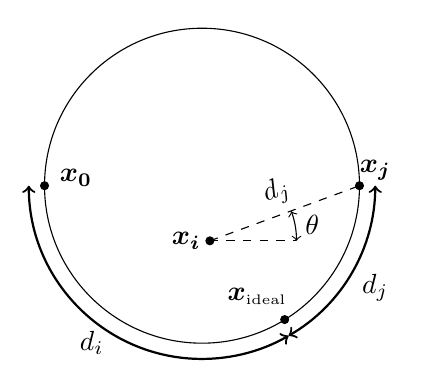
\begin{tikzpicture}
    \draw (2,0) circle(2);
    \filldraw (0,0) circle(0.05);
    \node at (0.4,0.1) {$\bm{x_0}$};

    \draw[thick,<->] (-0.2,0) arc (180:300:2.2);
    \node at (0.6,-2) {$d_i$};
    \filldraw (3.05,-1.7) circle(0.05);

    \draw[thick,<->] (4.2,0) arc (0:-60:2.2);
    \node at (4.2,-1.3) {$d_j$};

    \filldraw (4,0) circle(0.05);
    \node at (4.2,0.2) {$\bm{x_j}$};

    \node at (1.8,-0.7) {$\bm{x_i}$};
    \node at (2.7,-1.4) {$\bm{x}_{\mbox{{\tiny ideal}}}$};

    \filldraw (2.1,-0.7) circle (0.05);

    \draw[dashed] (2.1,-0.7) -- (4,0) node[above,midway,sloped] {$d_j$};

    \draw[dashed] (2.1,-0.7) -- (3.2,-0.7);
    \draw[<->] (3.2,-0.7) arc(0:20:1.1);
    \node at (3.4,-0.5) {$\theta$};
  \end{tikzpicture}
  \caption{Important values for the algorithm \emph{Note: not to scale}}
  \label{fig:algvals}
\end{figure}

The next step is to utilize these equations to calculate $\theta$. At any point
along the algorithm, we are at some $\bm{x_i}$, and we have travelled a
distance, $d_i$. Figure~\ref{fig:algvals} should help to understand what exactly
the algorithm is attempting to achieve. The idea is this: if we have travelled
some distance $d_i$, then there is an $\bm{x}_{\mbox{{\tiny ideal}}}$ on then
``ideal'' loop. The arc between $\bm{x}_{\mbox{{\tiny ideal}}}$ and $\bm{x_0}$
will be of length $d_i$. The algorithm searches for a point $x_j$ such that the
arc between $\bm{x}_{\mbox{{\tiny ideal}}}$ and $\bm{x_j}$ will have the
\emph{same} distance as the line between $\bm{x_i}$ and $\bm{x_j}$. Fortunately,
we have framed the equations for calculating $\bm{x_j}$ in terms of the distance
travelled along the arc, and the distance between $\bm{x_i}$ and $\bm{x_j}$ can
easily be calculated using the pythagorean theorem. Note that we find $\bm{x_j}$
as follows:
\begin{align}
  x_j = \frac{d}{2\pi} ( & \cos( \frac{ 2 \pi }{ d } ( \min( d, d_i + d_j ) )
                                  + \phi ) \notag \\ & - \cos \phi ) + x_0
                                  \label{eq:xj} \\
  y_j = \frac{d}{2\pi} ( & \sin( \frac{ 2 \pi }{ d } ( \min( d, d_i + d_j ) )
                                  + \phi ) \notag \\ & - \sin \phi ) + y_0.
                                  \label{eq:yj}
\end{align}
To satisfy our constraint, we have
\begin{equation}
d_j = \sqrt{ ( x_j(d_j) - x_i )^2 + ( x_j(d_j) - x_i )^2 }. \label{eq:dj}
\end{equation}

\subsubsection{Finding $d_j$}
Obviously, this is a rather difficult equation to truly solve, so we must only
heuristically find a solution. Unfortunately, even the heuristic solution is
a difficult one for a few reasons. Most problematically, the sine and cosine
functions have up to two stationary points on the interval we are considering
and there may not be a solution of $d_j$ that will satisfy the equality.
Nonetheless, we will do our best to mitigate these issues and apply a good
heuristic to find $d_j$. First, we rearrange our equation so that we can apply
a root-finding approximation algorithm to it:
\[ f(d_j) = \sqrt{(x_j(d_j) - x_i)^2 + (y_j(d_j) - y_i)^2} - d_j. \]
This simply allows the $d_j$ we are looking for to be the zero of the function.
The first exciting bit of news is that for most solutions of this equation with
$d_j < d$, it will work out that $f(0) > 0$ and $f(d-d_i) < 0$.
We know that $f(0) \geq 0$ by the
positivity of norms, and the square root of the sum of the squares is the
euclidian norm. We also can be certain that $f(d-d_i) < 0$ since
the norm is also unable to change by more than the diameter
of the ideal loop, or even less based on the proximity of $x_i$ to the center of
the loop. In situations where $f(d-d_i) > 0$, we notice that the distance to the
start of the loop is further away than the amount of distance we have left to
travel; this means that we should just route back to the start anyways. As such,
we have bounds inside of which we know that there exists a solution. We apply
Brent's method, a robust root approximation algorithm, to determine the solution
inside of this zone. The idea behind Brent's method is to combine the bisection
method, the secant method, and inverse quadratic interpolation. Readers
unfamiliar with any of these techniques should refer to \mycite{wik:sec},
\mycite{wik:bisect}, \mycite{wik:invquad}, \mycite{wik:brent} for a brief
overview of the techniques. A more interested reader might consider
\mycite{sauanal} for an in-depth analysis of the techniques as well as some
context for using and understanding them. Some pseudocode is given for Brent's
Method in Algorithm~\ref{alg:brent}, with some helper functions in
Algorithm~\ref{alg:bhelp}. The idea
is this:

\begin{algorithm}[t]
  \caption{Using Brent's Method to find a zero of a function}
  \label{alg:brent}
  \begin{algorithmic}
    \Require $f(a_0)f(b_0) > 0$
    \Function{Brent}{$f : [a,b] \to \mathbb{R}$, $a_0$, $b_0$}
      \If{$|f(a_0)| < |f(b_0)|$}
        \State \Call{swap}{$a_0$,$b_0$}
      \EndIf
      \State $b_{k-1} \gets a_0$
      \State $B \gets$ True \Comment{bisected last time?}
      \While{$f(b_k) \not = 0$ {\bf and} $|b_k - a_k| > \epsilon$}
      \If{$|f(a_k)| < |f(b_k)|$}
        \State \Call{swap}{$a_k$,$b_k$}
      \EndIf
      \State $b_{k+1} \gets$\Call{inv\_quad\_interp}{$f,a_k,b_k,b_{k-1}$}
      \State $B$ $\gets$ \Call{nds\_bi}{$a_k$,$b_{k-2}$,$b_{k-1}$,$b_k$,$b_{k+1}$,$B$}
      \If{$B$} \Comment{use bisection method}
        \State $\displaystyle b_{k+1} \gets \frac{a_k+b_k}{2}$
      \EndIf
      \State $b_{k-2} \gets b_{k-1}$
      \State $b_{k-1} \gets b_k$
      \If{$f(a_k)f(s) < 0$}
        \State $b_k \gets s$
      \Else
        \State $a_k \gets s$
      \EndIf
      \EndWhile
    \EndFunction
  \end{algorithmic}
\end{algorithm}
\begin{algorithm}[t!]
  \caption{Helper functions for Brent's method} \label{alg:bhelp}
  \begin{algorithmic}
    \State \Comment{\emph{Determines whether to use bisection~~~~~~~}}
    \State \Comment{\emph{method or inverse quadratic~~~~~~~~~~~~~~~~~}}
    \State \Comment{\emph{interpolation~~~~~~~~~~~~~~~~~~~~~~~~~~~~~~~~~~~}}
    \Function{nds\_bi}{$a_k$,$b_{k-2}$,$b_{k-1}$,$b_k$,$b_{k+1}$,$B$}
      \If{$\displaystyle b_{k+1} \not \in \left[ \frac{3a_k+b_k}{4},b_k \right]$}
      \State \Return True
      \ElsIf{$B$ is True}
      \State \Return
        $\displaystyle |b_{k+1}-b_k| \geq \frac{|b_k-b_{k-1}|}{2}$
      \State ~~~~~~~~~~~$\land$~~$|b_k-b_{k-1}| < |\delta|$
      \Else
      \State \Return $\displaystyle |b_{k+1}-b_k| \geq \frac{|b_{k-1}-b_{k-2}|}{2}$
      \State ~~~~~~~~~~~$\land$~~$|b_{k-1}-b_{k-2}| < |\delta|$
      \EndIf
    \EndFunction
  \end{algorithmic}
  \begin{algorithmic}
    \State \Comment{\emph{returns the next iterate under inverse~~~~~}}
    \State \Comment{\emph{quadratic interpolation~~~~~~~~~~~~~~~~~~~~~~~~~}}
    \Function{inv\_quad\_interp}{$f$,$a$,$b$,$c$}
      \If{$f(a) \not= f(c)$ {\bf and} $f(b) \not= f(c)$}
        \State \Return $\displaystyle \frac{af(b)f(c)}{(f(a)-f(b))(f(a)-f(c))}$
        \State ~~~~~~~~~~~$\displaystyle + \frac{bf(a)f(c)}{(f(b)-f(a))(f(b)-f(c))}$
        \State ~~~~~~~~~~~$\displaystyle + \frac{cf(a)f(b)}{(f(c)-f(a))(f(c)-f(b))}$
      \Else
        \State \Return $\displaystyle b - f(b)\frac{b-a}{f(b)-f(a)}$
      \EndIf
    \EndFunction
  \end{algorithmic}
\end{algorithm}

First, we need a bracket in which our function has a root. For us, this is
simple enough; we just use $[0, d-d_i]$. If that bracket does not satisfy the
condition, we just set $d_j = d-d_i$ and don't bother with anything.

The algorithm details out the actual swapping of $a_k$ and $b_k$, but here
we'll just assume that $|f(a_k)| > |f(b_k)|$ at all points in time; that is,
$b_k$ is a better approximation of the solution than $a_k$. We also require
$b_{k-1}$; at the beginning, $a_k$ will suffice instead.

This is a heuristic, so we'll keep repeating the algorithm until either
$a_k \approx b_k$ or $f(b_k) \approx 0$. At the $k^{\mbox{{\tiny th}}}$ iteration,
we'll calculate $b_{k+1}$ using both inverse quadratic interpolation and the
bisection method.

In general, the inverse quadratic interpolation can proceed very quickly, but we
add the bisection method to ensure convergence. In order to use interpolation,
we require that a few conditions are satisfied. Namely, $s$ has to be in a certain
interval, and the iterates need to obey certain bounds.

The rest of the pseudocode serves only to ensure that variables are assigned
correctly. One notes that $B$ indicates whether the bisection method was used
on the previous iteration.

Thus, by utilizing Brent's Algorithm, we can find $x_j$. From here, calculating
$\theta$ is fairly straightforward:
\begin{align}
  \tan \theta = & \frac{y_j - y_i}{x_j-x_i} \notag \\
  \theta = & \tan^{-1} \frac{y_j - y_i}{x_j-x_i} \label{eq:theta}
\end{align}

Finally, we have a method for calculating the weights based on distance and
direction! Use Brent's algorithm as described in Algorithm~\ref{alg:brent}
with the function to be zeroed as \eqref{eq:dj}. Use that $d_j$ in conjunction
with \eqref{eq:xj} and \eqref{eq:yj} to find
$x_j$ and $y_j$, respectively, and plug into \eqref{eq:theta} to find a
$\theta$. Finally, use $\theta$ in conjunction with \eqref{eq:weight} to assign
weights to directions.

\subsection{Miscellaneous Weights}

There are a few more important characteristics to consider when calculating
weights. Perhaps the easiest of these to deal with are the built in road types
that the Open Street Map format provides. It is easy enough to assign these
priorities based on what a cyclist would reasonably hope to see. Basically,
busy roads get weighted lower than low-traffic roads, but things like
pedestrian walkways and other unridable roads also get high weights.
Interestingly, pyroute already sets weights for these values, but these are
generated based on preferences for navigating; these vary greatly from
preferences for going out and having a good time. A good example of this is the
weight that pyroute assigns for cycling on steps, which is not 0. It is
certainly possible for the cyclist to dismount and climb the steps, but one who
is riding for fun is highly unlikely to be excited about this prospect.

Another characteristic to consider is whether a road has already been
travelled. Repeatedly riding along the same stretch of road can make a ride
rather boring, so by weighting against this, it can be avoided. In order to deal
with this, the algorithm stores stretches of road that have been travelled and
halves the weight of any path that the rider has already ridden.

\subsection{Using the Weights to Generate a Route}

Now that we have developed all of the weight calculations, we can consider using
them to generate a route. Algorithm~\ref{alg:grow} lays out the basic idea in
pseudocode. It omits definitions for many of the functions because they were
covered in sufficient detail in previous sections. In particular the function
for calculating weights is omitted, but it utilizes the algorithms and
characteristics discussed in previous sections
The general procedure is
to loop until the algorithm returns to the start point after at least 90\%
of the distance, $d$ is travelled. At each iteration, $\theta$ will be
calculated using \eqref{eq:theta}, where $(x_j,y_j)$ are calculated by applying
Algorithm~\ref{alg:brent} on \eqref{eq:dj}. Once $\theta$ is calculated, a
weight is generated for each node adjacent to $x_i$, and one of the nodes is
selected at random based on their weights.

\begin{algorithm}[t!]
  \caption{Calculating a Route} \label{alg:grow}
  \begin{algorithmic}
    \Require \Call{edges}{} finds adjacent nodes and \Call{random}{} generates
    a random number in the given range.
    \Function{grow\_cycle}{$x_0$,$d$,$e$,$\phi$}
    \State $X \gets \{\}$ \Comment{the route}
    \State $d_k \gets 0$
    \State $\theta \gets \phi$

    \While{$x_{k}\not = x_0$ {\bf or} $d_k < 0.9d$}
      \State $\theta \gets$ \Call{get\_theta}{}

      \State $w \gets 0$ \Comment{sum of all weights}
      \For{$x \in$ \Call{edges}{$x_k$}}
        \State $w \gets w +$\Call{weight}{$x$,$\theta$}
      \EndFor
      \State $q \gets$ \Call{random}{$[0,w]$}
      \For{$x \in$ \Call{edges}{$x_k$}}
        \If{$q < $ \Call{weight}{$x$,$\theta$}}
          \State $x_{k+1} \gets x$
          \State $d_{k+1} \gets d_k +$\Call{dist}{$x_k$,$x_{k+1}$}
          \State $X \gets X \cup \{x_{k+1}\}$
          \State break
        \Else~$q \gets q -$\Call{weight}{$x$,$\theta$}
        \EndIf
      \EndFor
    \EndWhile
    \State \Return $X$
  \EndFunction

  \end{algorithmic}
\end{algorithm}

\section{Using Spherical Coordinates} \label{sec:latlong}

As mentioned earlier, using the Euclidian norm for latitudes and longitudes
is inaccurate; latitudes and longitudes are spherical coordinates  with
fixed $r$. As one can see in Figure~\ref{fig:sphere},
spherical coordinates are the three dimensional
equivalent of polar coordinates. Unfortunately, this poses two problems,
since we have only described generating a route around the origin in a two
dimensional plane. The first problem is switching to a spherical coordinate
system; the second is switching to three dimensions. Clearly,
considering the latitude and longitude to be values on a cartesian
coordinate plane is a flawed idea. Latitudes and longitudes are angles, not
positions in space.

\begin{figure}
  \centering
  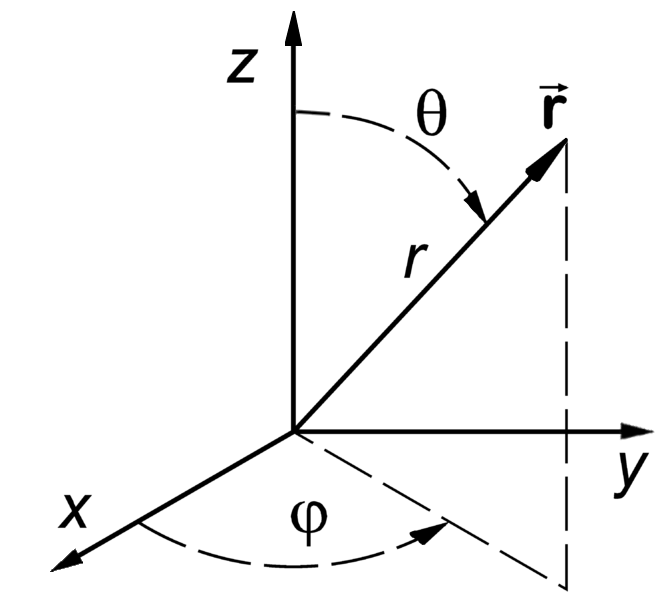
\includegraphics[height=2in]{images/sphere.png}
  \caption{The Spherical Coordinate System~\mycite{img:spher}} \label{fig:sphere}
\end{figure}

\subsection{Distance Calculations}
Fortunately, distances are very well defined under any coordinate system, so we
can tackle both problems here without much ado. In the spherical coordinate
system, The haversine formula is used to calculate distances between two points
on the surface of a sphere. The haversine formula uses the haversin function,
which is defined as follows:
\newcommand{\haversin}{\mbox{haversin}}
\[ \haversin (\theta) = \sin^2(\frac{\theta}{2}). \]
Given two coordinate pairs, $(\phi_1, \lambda_1)$ and $(\phi_2, \lambda_2)$,
and a radius, $r$, the haversine formula calculates the distance $d$ between
the two coordinate pairs \mycite{wik:haversin}:
\begin{align*}
  d = r\haversin^{-1}(&\haversin(\phi_2 - \phi_1) + \\
  & \cos(\phi_1)\cos(\phi_2)\haversin(\lambda_2 -\lambda_1)
\end{align*}
Using the definition of the haversin function, this can be reduced into a
function in terms of elementary trigonometric functions. The only non-trivial
thing to note is that $\haversin^{-1}(x) = 2\sin^{-1}(\sqrt{x})$. Armed with
this knowledge, it is fairly easy to reduce. We'll use an intermediate variable
to hold the value under the square root:
\begin{align*}
  h = & \haversin(\phi_2-\phi_1) + \\
  & \cos(\phi_1)\cos(\phi_2)\haversin(\lambda_2-\lambda_1) \\
  = & \sin^2\left(\frac{\phi_2 - \phi_1}{2}\right) + \\
  & \cos(\phi_1)\cos(\phi_2)\sin^2\left(\frac{\lambda_2-\lambda_1}{2}\right)\\
  d = & r\haversin^{-1}\left(\sqrt{h}\right) \\
  = & 2r\sin^{-1}\left(\sqrt{h}\right)
\end{align*}
By simply substituting this as the right hand side of \eqref{eq:dj}, many of the
projection issues can be avoided.

 However, it still isn't perfect; the haversine
formula does not account for variations in the elevation of the earth. Instead,
it assumes one is travelling at sea level. Additionally, it assumes the earth is
a perfect sphere, which is also slightly inaccurate. Less accurate formulae
include flat-surface projection formulae, while more accurate formulae
generate geodesics along the surface of an ellipsoid that models the earth
\mycite{wik:dist}. For our purposes, however, the haversine formula will be
sufficiently accurate.

\subsection{Ideal Loop Calculation}

Distance calculations are the easier half of the problem;
the actual ideal loop and, consequently,
\eqref{eq:xj} and \eqref{eq:yj} depend on a set of parametric equations along
a cartesian coordinate plane. We'll consider a few different methods for
converting to spherical coordinates.

\subsubsection{A Na\"{i}ve Approach} \label{sec:naiveloop}

The first, and perhaps most obvious, method is to simply use latitude and
longitude as the $x$ and $y$ in \eqref{eq:xj} and \eqref{eq:yj}. This is
not a superb solution, but it does have a few advantages, chief of which are
the relative ease of computation and development. For small loops relatively
close to the equator, it may even be fairly similar to the intended ideal loop.

However, the larger the loop and the further from the equator the more squashed
the loop will begin to be. One also notes that the conversion does require a
slight change to the original formulae: one cannot use $d$ as the radius of the
circle. Instead, one must use an approximate conversion of the input distance
to an angular delta. Latitudinal distances change very little (they only
change because the Earth is an ellipsoid, not a sphere), and, as such, the
nautical mile was derived as the distance between a minute of latitude
\mycite{wik:nautmil}. Thus, we can easily convert between a distance goal and an
approximate latitudinal radius. Unfortunately, this will be dramatically
incorrect the closer to the poles we get.

\subsubsection{Accurate Approach}

\begin{figure}
  \centering
  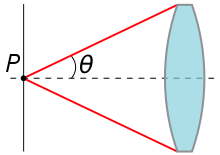
\includegraphics[width=2in]{images/220px-Numerical_aperture.png}
  \caption{The half-aperture of a cone \mycite{img:aperture}} \label{fig:aperture}
\end{figure}

To find the real ideal loop, a cone must be projected from the origin of the
sphere, and the intersection of the cone and the sphere can be used to calculate
the ideal loop. Note that this approach, while far superior to the flattened
approach, still does not compensate for the ellipsoidal nature of the Earth, or
for the variations in the elevation on the surface of the earth.

The following equation describes a cone:,
\[ 0 = (\bm{u} \cdot \bm{d})^2 - |\bm{d}|^2|\bm{u}|^2\cos^2 \phi , \]
where $\bm{u}= (x,y,z)$, $\bm{d} = (a,b,c)$ is a vector parallel to the axis of
the cone, and $\phi$ is one-half the aperture of the cone \mycite{wik:cones}. In
Figure~\ref{fig:aperture}, the $\theta$ pictured is the same as the $\phi$ in
this equation; we have used $\phi$ instead of the more accepted $\theta$ to
avoid confusion with the zenith in spherical coordinates.
Additionally, recall the equation for a sphere:
\[ r = |\bm{u}|. \]
For the most part, we can consider $r = 1$, since we are dealing with the
surface of a sphere. However, we do have to make certain calculations using
the actual radius of the earth. For example, in order to calculate the
aperture $\phi$, we realize that the length of the sides of the cone will be the
radius of the earth. Then $\sin \phi = \frac{r_c}{r}$, so we can calculate
$\phi$ as follows:
\begin{equation}
  \phi = \sin^{-1} \left( \frac{\frac{d}{2\pi}}{r} \right) \label{eq:phi}
\end{equation}

With $r = 1$, we do our best to create an equation for the circle of interest:
\begin{align*}
  0 = & (\bm{u}\cdot \bm{d})^2 - |\bm{d}|^2|\bm{u}|^2\cos^2 \phi \\
    = & (ax + by + cz)^2 - \cos^2 \phi \\
    = & a^2x^2 + b^2y^2 + c^2z^2 \\
    & + 2abxy + 2acxz
     + 2bcyz - \cos^2 \phi \\
\end{align*}

Unfortunately, these equations for spheres and cones are of little aid. The
 parametric equations for a circle are inspired by the polar coordinate form
of a circle, so we convert these equations to spherical form. Ideally, this will
likewise inspire a set of parametric equations for this circle.
\begin{align*}
  0 = & a^2x^2 + b^2y^2 + c^2z^2 \\
      & 2abxy + 2acxz + 2bcyz - \cos^2 \phi \\
    = & a^2\cos^2 \psi + b^2\sin^2 \psi + c^2\sin^2 \theta \\
      & + 2ab\cos \psi\sin \psi + 2ac\cos \psi \sin \theta \\
      & + 2bc\sin \psi \sin \theta  - \cos \phi
\end{align*}
Unfortunately, this doesn't make much headway. Without further inspiration,
we'll stick with the na\"{i}ve approach discussed in
Section~\ref{sec:naiveloop}.

\section{Experimentation \& Results}

At first, the algorithm was rather unsuccessful. The generated weights may have
been useful, but a few things kept them from being very successful. First, the
weights were calculated at every node. This means that at every point along a
road, it would be determined if one should continue down the road or turn around
and head back in the other direction. Unfortunately, since many roads are rather
curvy, the weights could often tell the user to oscillate back and forth on a
single road for an entirely uninteresting ride.

In subsequent iterations of the algorithm, this was noticed and adjusted for;
instead, the next intersection is found, and the weights are calculated for the
point at the next intersection. This also allows for weights for previously
travelled sections of road to be compressed to pairs of nodes for each stretch
between an intersection.

Another issue arose with the preliminary calculation of $\theta$. At first, a
much more na\"{i}ve approach was taken. Instead of using Brent's method to find
the zeroes of \eqref{eq:dj}, the algorithm simply divided the search space into
one hundred sections and chose the section that was closest. 

Another difficult issue was getting the algorithm to terminate. Sometimes the
algorithm might get stuck in a dead end where $x_0$ is a straight line through
the dead end as the crow flies, so the algorithm weights continuing down the
dead end higher. Even if something like this did not happen, the loops were
almost invariably well above the distance input. In order to avoid this problem,
the algorithm utilizes point-to-point routing to route back to the start once
$d_i + \|\bm{x}_0-\bm{x}_i\| > 0.95d$; that is, once the direct distance between
the current point and the starting point summed with the distance travelled is
more than 95\% of the distance goal. This allows for both flexibility and
variation. If the route back to the starting point is direct, the loop will be
somewhat below the desired distance goal. On the other hand, if the route back
to the starting point is less direct, the loop will slightly exceed the input
distance goal.

\section{Future Work}

There are many ways to expand the algorithm developed here. While we have done
our best to utilize as much data as possible, expanding the set of data utilized
to generate the routes will likely improve the algorithm. Additionally, some
features were abandoned due to time constraints.

Unfortunately, the API we used for OSM did not have easy access to elevation
data, something that would have also proved very useful to cyclists. A more
robust implementation of this algorithm would also find the elevation data of
every coordinate and use this information to augment the weights. This would
also give rise to some very interesting challenges due to the competing
interests of elevation and distance.

There has been research done into analyzing the probability of accidents
on a road based on certain metadata. This metadata is readily available to the
cities that maintain the roads, but it is beyond the scope of the information
contained in OSM data or even better-funded mapping applications such as
Google Maps. Ideally, as time progresses the data will percolate into these
services; if this data becomes more readily available, then it can be integrated
into the algorithm to help increase user safety.

Additionally, this has been a facet of a three pronged project developing an
immersive experience for bicycle training. The other two prongs are an
Android application to track training data during a ride and a website to track
long-term training data. Ideally, this algorithm will eventually be seamlessly
integrated into the mobile and web projects, so that routes can be generated
on the web and sent directly to the user's mobile phone for the user to follow
with the Android application.

Once the three prongs of this project have been integrated together, leveraging
the data from the other parts would also provide valuable input for the
algorithm. As mentioned in Section~\ref{sec:back}, cyclists generally perform
their own version of this algorithm to find routes that they will enjoy. Once
the web experience is fully fleshed out users will upload all of their rides
to the website so that they can be viewed and analyzed in the future. This also
provides extremely valuable data for the algorithm, since user generated routes
may favor better, more interesting roads than a purely weight driven experience.
With this data, the algorithm could add a ``heatmap'' layer to the algorithm
that keeps track of how popular a road is. Roads that are seldom used could be
weighted negatively, while extremely popular roads would be almost mandatorily
included in generated routes.

Another valuable extension would be to generate routes that are not necessarily
circuits. In this paper, we have focused on loops since cyclists are likely to
want to return home after a good training ride. However, it might also be useful
to have some sort of quasi-navigation that aims for the most fun route
between two locations rather than the most direct route. This way, riders might
be able to mix commute and training.

Additionally, it might be worthwhile to explore other methods for generating
routes. A weight based algorithm makes randomization fairly easy, but other
concepts certainly exist. Another idea might be to just take a
breadth-first-search that returns to the start and choose at random one of the
solutions that is within some epsilon of the distance goal. This approach may
be a pretty solid one, but it does raise some challenges when extended for
additional goals, and enumerating all possibilities may prove computationally
taxing, especially if space constraints become an issue.

\bibliographystyle{plainnat}
\raggedright
\bibliography{paper}

\end{document}
